\subsection{Tecnología}

\subsubsection{Infraestructura}
El punto de vista de Infraestructura contiene los elementos de infraestructura de software y hardware que soportan la capa de aplicación, como dispositivos físicos, redes o software del sistema (por ejemplo, sistemas operativos, bases de datos y middleware).
\paraghap{Modelo}
\begin{figure}[h!]
	\centering
	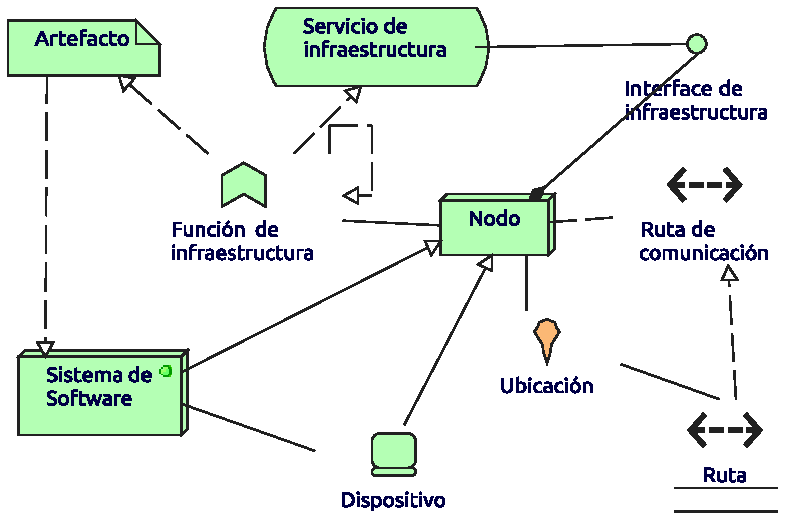
\includegraphics[width=0.8\linewidth]{Desarrollo/ArquitecturaEmpresarial/Tecnologia/imgs/insfraestructuraMetamodelo.pdf}
	\caption{Organización}
\end{figure}
\newpage
\paraghap{Caso de Estudio}

\begin{figure}[h!]
	\centering
	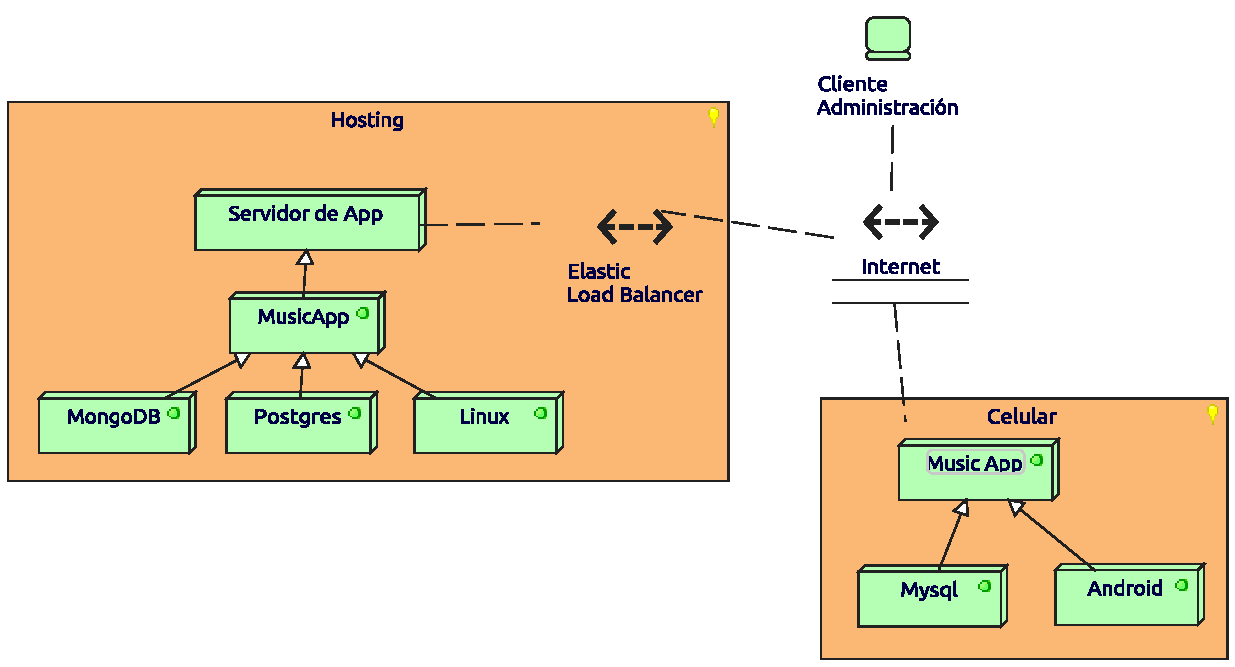
\includegraphics[width=\linewidth]{Desarrollo/ArquitecturaEmpresarial/Tecnologia/imgs/insfraestructura.pdf}
	\caption{Caso}
\end{figure}

\newpage

\subsubsection{Uso de Infraestructura}
\paraghap{Modelo}
\begin{figure}[h!]
	\centering
	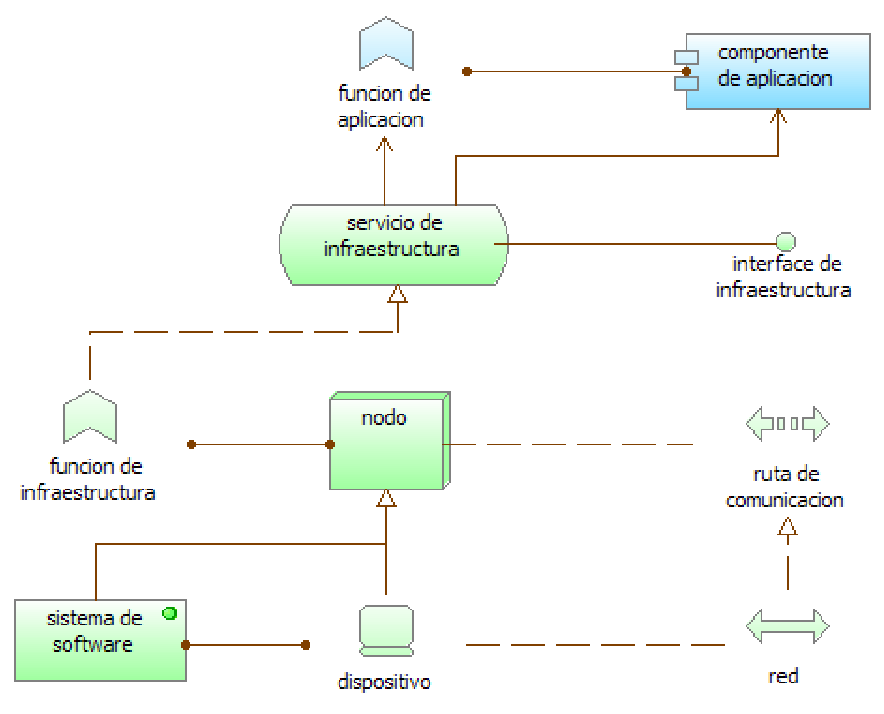
\includegraphics[width=0.8\linewidth]{Desarrollo/ArquitecturaEmpresarial/Tecnologia/imgs/uso.PNG}
	\caption{Organización}
\end{figure}
\newpage
\paraghap{Caso de Estudio}

\begin{figure}[h!]
	\centering
	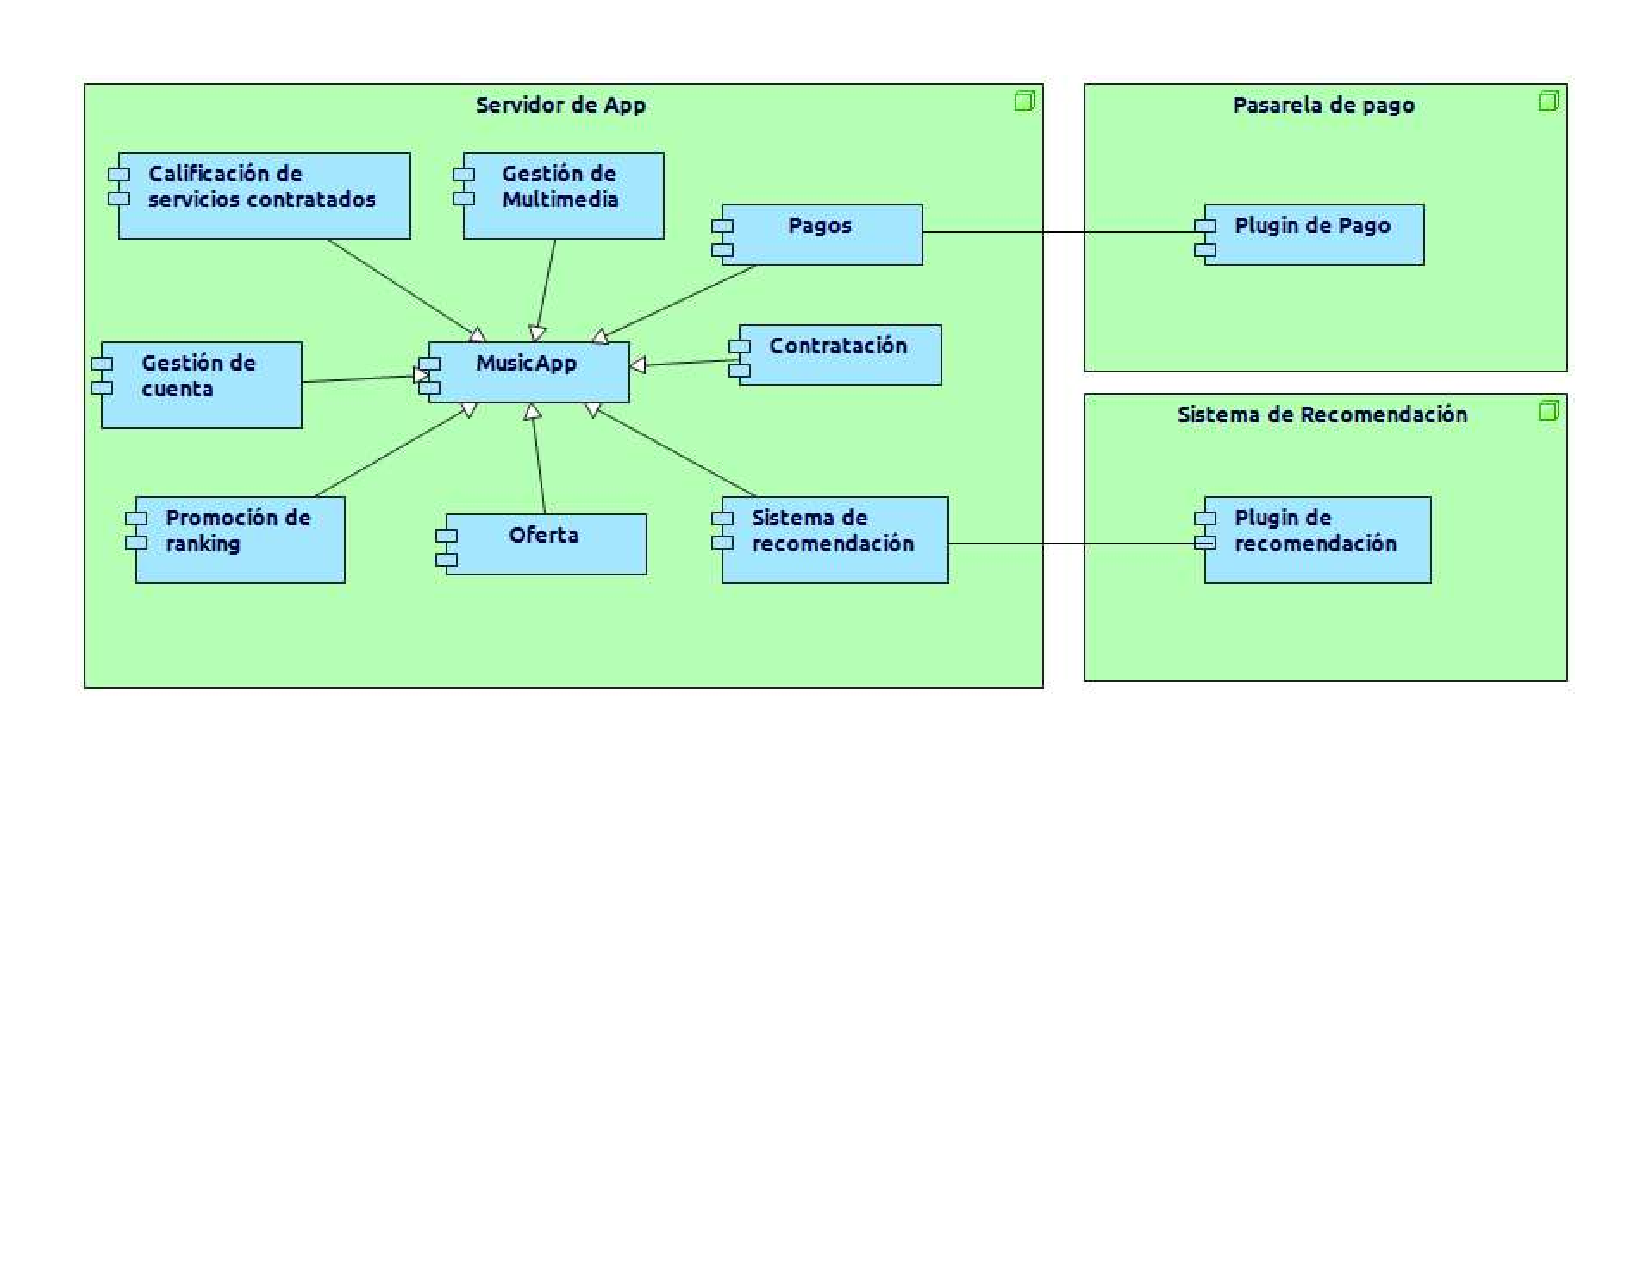
\includegraphics[width=\linewidth]{Desarrollo/ArquitecturaEmpresarial/Tecnologia/imgs/uso.pdf}
	\caption{Caso}
\end{figure}

\newpage

\subsubsection{Estructura de Información}
\paraghap{Modelo}
\begin{figure}[h!]
	\centering
	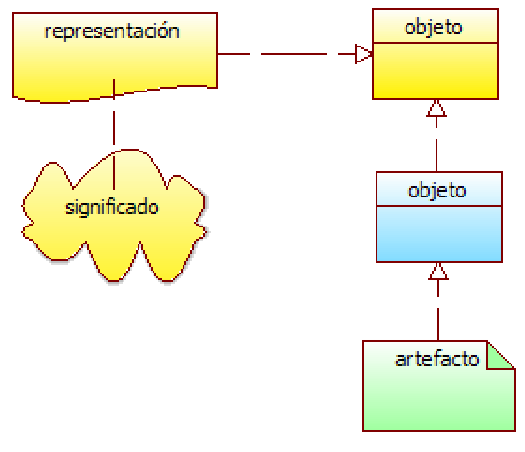
\includegraphics[width=0.8\linewidth]{Desarrollo/ArquitecturaEmpresarial/Tecnologia/imgs/estructuraMetamodelo.PNG}
	\caption{Organización}
\end{figure}
\newpage
\paraghap{Caso de Estudio}

\begin{figure}[h!]
	\centering
	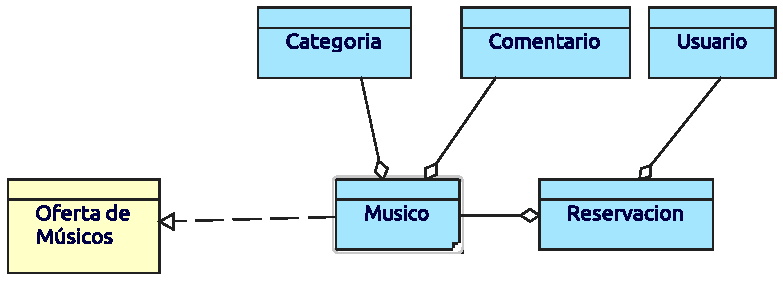
\includegraphics[width=\linewidth]{Desarrollo/ArquitecturaEmpresarial/Tecnologia/imgs/estructura.pdf}
	\caption{Caso}
\end{figure}

\newpage

\subsubsection{Realización del servicio}
\paraghap{Modelo}
\begin{figure}[h!]
	\centering
	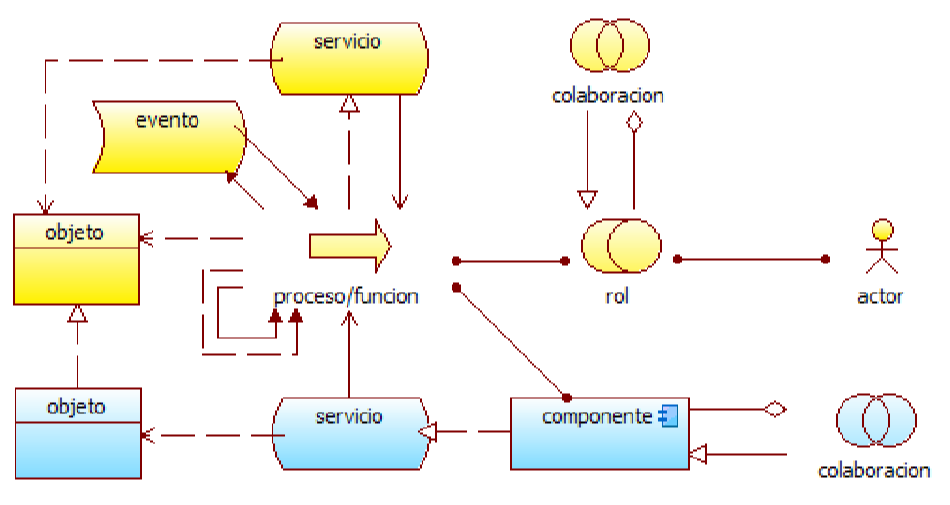
\includegraphics[width=\linewidth]{Desarrollo/ArquitecturaEmpresarial/Tecnologia/imgs/realizacionMetamodelo.PNG}
	\caption{Organización}
\end{figure}
\newpage
\paraghap{Caso de Estudio}

\begin{figure}[h!]
	\centering
	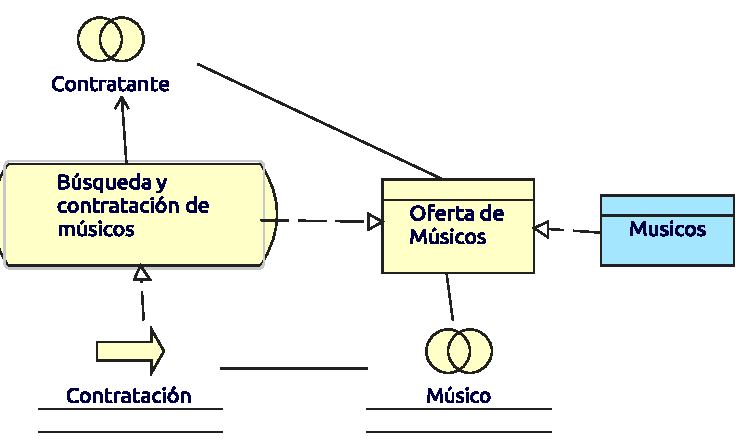
\includegraphics[width=\linewidth]{Desarrollo/ArquitecturaEmpresarial/Tecnologia/imgs/realizacion.pdf}
	\caption{Caso}
\end{figure}

\newpage

\subsubsection{Capas}
\paraghap{Modelo}
Todos los conceptos y todas las relaciones.
\paraghap{Caso de Estudio}

\begin{figure}[h!]
	\centering
	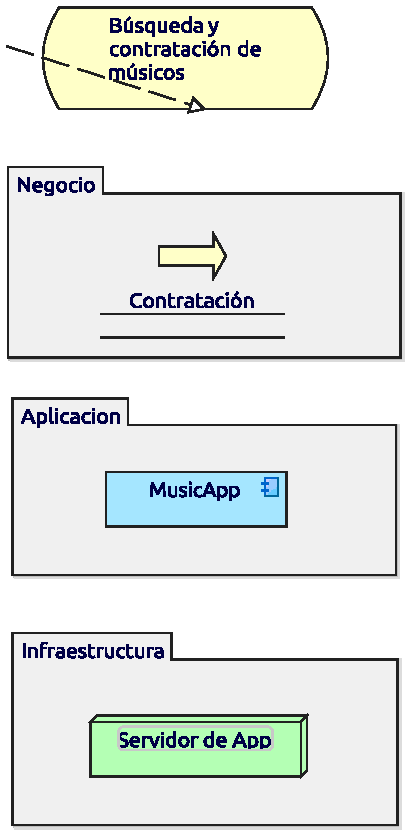
\includegraphics[width=0.5\linewidth]{Desarrollo/ArquitecturaEmpresarial/Tecnologia/imgs/capas.pdf}
	\caption{Caso}
\end{figure}

\newpage